\section{Results}

\subsection{Clean-v3 validation comparison}


\begin{table*}[t]
\centering
\caption{Clean-v3 validation point estimates under the older geometry contract. Both rows are single-run validation evidence; no confidence interval or protected-test result is available.}
\label{tab:clean-v3-validation}
\begin{tabular}{lrrrrr}
\toprule
Model & Robust Dice & Robust IoU & Precision & Recall & BF1 \\
\midrule
IMP-SegFormer-B3 & 0.8959 & 0.8277 & 0.9088 & 0.9128 & 0.4145 \\
nnU-Net v2 & 0.9019 & 0.8354 & 0.9056 & 0.9246 & 0.4369 \\
\bottomrule
\end{tabular}
\end{table*}


nnU-Net v2 has the higher recorded robust-Dice point estimate: 0.9019 versus 0.8959 for \impmodel{}. Its boundary F1 and recall have higher recorded point estimates, while the IMP control has slightly higher precision. These directions suggest an overlap--precision trade-off, but adaptive use of validation, the lack of repeated seeds, and unavailable paired confidence intervals prevent a statistical-superiority conclusion.

The result also does not authorize test-v3 access under the historical combined gate. The correct statement is therefore narrow: under the legacy geometry contract, nnU-Net has higher recorded \cleanv{} validation point estimates for robust Dice and boundary F1. These single-run observations are not a superiority conclusion.

\subsection{Three-seed contour-channel ablation}


\begin{table}[t]
\centering
\caption{Loop206 contour-channel minus zero-channel control on the train-screen protocol with three paired seeds, 76 groups, and 10,000 cluster-bootstrap resamples.}
\label{tab:loop206-ablation}
\begin{tabular}{lrr}
\toprule
Metric & Point delta & 95\% CI \\
\midrule
Robust Dice & -0.0313 & [-0.0491, -0.0156] \\
Boundary F1 & -0.0147 & [-0.0308, 0.0010] \\
\bottomrule
\end{tabular}
\end{table}



\begin{table*}[t]
\centering
\caption{Loop206 gate audit derived only from the hash-bound closure receipt. Every reported interval is conditional on the three selected seeds. Missing receipt fields remain \texttt{unavailable} and force \texttt{blocked} rather than reconstructing a gate decision.}
\label{tab:loop206-gate-audit}
\scriptsize
\def\sidprefix{seed-}
\resizebox{\textwidth}{!}{%
\begin{tabular}{llllllllll}
\toprule
gate\_id & endpoint & threshold & observed & interval & \sidprefix206 & \sidprefix1206 & \sidprefix2206 & status & source \\
\midrule
primary\_improvement & robust Dice delta &
unavailable & -0.0313 & [-0.0491, -0.0156] & unavailable & unavailable & unavailable & blocked & loop206\_report@7d6fcd61259a \\
dice\_noninferiority & robust Dice delta &
unavailable & -0.0313 & [-0.0491, -0.0156] & unavailable & unavailable & unavailable & blocked & loop206\_report@7d6fcd61259a \\
boundary\_noninferiority & boundary F1 delta &
unavailable & -0.0147 & [-0.0308, 0.0010] & unavailable & unavailable & unavailable & blocked & loop206\_report@7d6fcd61259a \\
clean\_dice & unavailable &
unavailable & unavailable & unavailable & unavailable & unavailable & unavailable & blocked & loop206\_report@7d6fcd61259a \\
precision & robust precision delta &
unavailable & -0.0201 & unavailable & unavailable & unavailable & unavailable & blocked & loop206\_report@7d6fcd61259a \\
recall & robust recall delta &
unavailable & -0.0142 & unavailable & unavailable & unavailable & unavailable & blocked & loop206\_report@7d6fcd61259a \\
distance & HD95 and ASSD deltas &
unavailable & 7.7911 / 5.0786 & unavailable & unavailable & unavailable & unavailable & blocked & loop206\_report@7d6fcd61259a \\
per\_corruption & unavailable &
unavailable & unavailable & unavailable & unavailable & unavailable & unavailable & blocked & loop206\_report@7d6fcd61259a \\
\bottomrule
\end{tabular}%
}
\end{table*}


\begin{figure}[t]
\centering
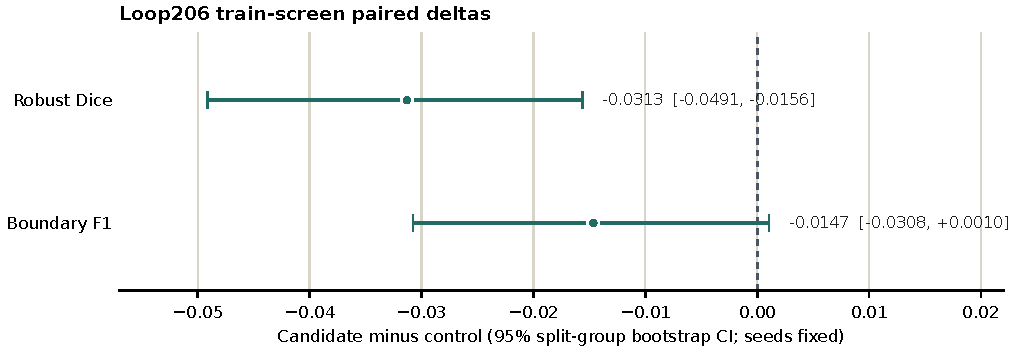
\includegraphics[width=\linewidth]{figures/loop206_delta.pdf}
\caption{Loop206 candidate-minus-control deltas on the \texttt{train\_screen} protocol with 95\% split-group cluster-bootstrap confidence intervals after averaging selected seeds and views. The intervals are conditional on those seeds. The zero line marks no paired change. Loop191 and Loop192 point estimates are excluded because paired confidence intervals are unavailable for those runs.}
\label{fig:loop206-delta}
\end{figure}

After averaging the three selected seeds and three views, the contour channel changes robust Dice by $-0.0313$. Its conditional 95\% split-group bootstrap interval, $[-0.0491,-0.0156]$, lies entirely below zero. Per-seed directions are unavailable in the authorized closure receipt, so the aggregate statement must not be read as a reduction in every seed. On this 76-group train-screen protocol, the aggregate result contradicts the stated positive primary-effect requirement; it does not establish a broader claim about contour methods or seed-population uncertainty. Boundary F1 changes by $-0.0147$; its interval $[-0.0308,0.0010]$ includes zero, providing no evidence of the intended boundary benefit. Precision and recall also decline in the recorded aggregate, while HD95 and ASSD increase.

The authorized closure receipt records only the global decision \texttt{gate\_passed=false}, establishing that at least one preregistered gate did not pass; it does not enumerate individual gate decisions. Table~\ref{tab:loop206-gate-audit} exposes the fixed eight-gate contract without reconstructing those decisions. Every interval is conditional on the selected seeds. Thresholds, per-seed directions, and unreported endpoints are \texttt{unavailable}, so every individual gate status remains \texttt{blocked}. Clean-v3 validation, test-v3, and PH2 remain sealed. The operational default and scientific reference are unchanged.

\subsection{Fixed-cache qualitative demonstration}

Figure~\ref{fig:qualitative-demo} shows three clean, non-protected examples selected without prediction or metric inspection: the first, middle, and last rows after sorting all 76 train-screen rows by sample identifier and group key. Each comparison was produced by the real GPU service and has a path-free receipt labeled \texttt{train\_screen}, \texttt{exact\_fixed\_cache}, and \texttt{historical\_cache\_provenance\_drift}. Ground truth appears only after the pinned provenance manifest verifies source identity, raw and decoded image hashes, CC-0 image license, and challenge ground-truth status. Mask bytes are separately bound to the pinned dataset index by raw, decoded-binary, and runtime digests before rendering. The panels illustrate mask geometry and disagreement; they do not estimate generalization or authorize arbitrary-upload candidate inference.

\begin{figure*}[t]
\centering
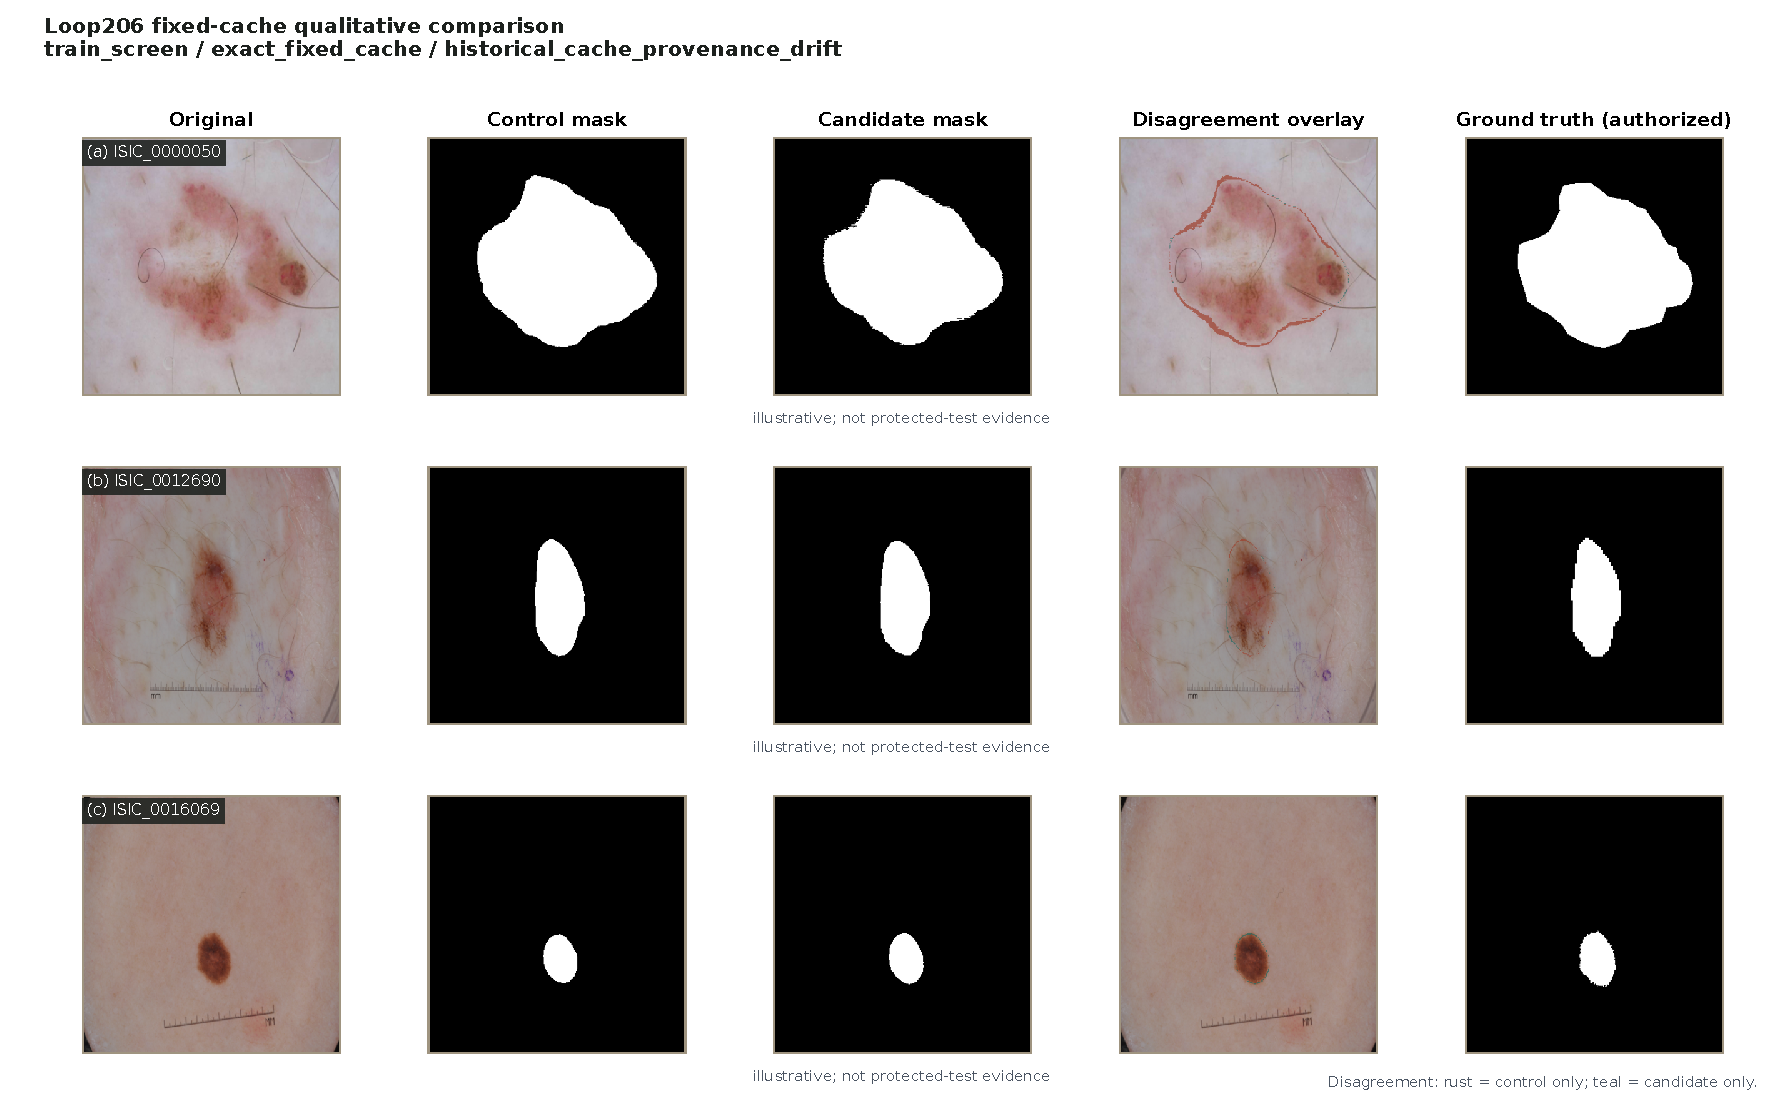
\includegraphics[width=\textwidth]{figures/qualitative_demo.pdf}
\caption{Three deterministic, non-protected fixed-cache comparisons. Columns show the original image, control mask, candidate mask, disagreement overlay, and authorized train-screen ground truth. Rust marks control-only pixels and teal marks candidate-only pixels. Each of the 15 modality subplots visibly carries the exact notice \texttt{illustrative; not protected-test evidence}.}
\label{fig:qualitative-demo}
\end{figure*}

\subsection{Bounded live dual demonstration}

Live L206-control-s206 versus a reconstructed Loop192 runtime is an illustrative, metric-free display; it does not reproduce the Loop191-versus-Loop192 Paper RQ1 comparison. In shorthand, it does not reproduce the Loop191-versus-Loop192 RQ1 comparison. The runtime is identified as L192-nnUNet-v2-raw-100ep. The service sequences independent copies of the same public or synthetic RGB input through L206 first and reconstructed L192 second; this execution order does not make either model an input to the other. A receipt is eligible only after both arms succeed and bind their model, checkpoint, input, and mask hashes. No canonical live runtime receipt is included at this stage. Ground truth is not loaded or used. Accuracy is not measured or claimed. The Live dual demo reports no metric for this live path. Its masks are illustrative.

\paragraph{Evidence classification.} Observed: the historical Task 4 resume report records bounded loopback sidecar/Gradio inference, fail-closed oversized input, retry/recovery, desktop 1440x900 and mobile 390x844 browser checks, and an ephemeral Cloudflare public GET. That historical report is not current-release acceptance evidence. Current-release browser, mobile/desktop visual, and tunnel status is \texttt{unverified/blocked}: the canonical blocked packet at \texttt{demo\_runtime/acceptance/imp.dual\_live.e2e.v1/20260722T233947051Z/acceptance.json} omits browser/tunnel fields, and the Presenter S transcript records browser discovery failure. Established: historical operational observations support only their stated checks; they do not support ground-truth accuracy or original-runtime equivalence. Assumption: no live receipt is promoted into the release, so the live lane remains separate from fixed-cache and Paper RQ1 evidence. Speculation: no causal, clinical, or superiority property follows from illustrative live masks. The historical Task 4 report recorded an 83-mask-pixel reconstructed-runtime repeat drift under matched bindings; that bounded historical observation is not current-release determinism acceptance, which remains blocked.

\subsection{Legacy comparison}


\begin{table*}[t]
\centering
\caption{Legacy Clean-v2 test-v2 values. Evidence class: \texttt{legacy\_patient\_contaminated}. Three patient IDs and 13 rows participate in cross-split contamination; these values are historical only.}
\label{tab:legacy-loop170}
\begin{tabular}{lrrrr}
\toprule
Model & Robust Dice & Clean Dice & Robust IoU & BF1 \\
\midrule
EGE-UNet & 0.8616 & 0.8617 & 0.7809 & 0.0817 \\
IMP-SegFormer-B3 & 0.8913 & 0.8962 & 0.8224 & 0.4240 \\
Vanilla SegFormer-B3 & 0.8897 & 0.8968 & 0.8179 & 0.3969 \\
nnU-Net v2 & 0.8911 & 0.8923 & 0.8246 & 0.5381 \\
\bottomrule
\end{tabular}
\end{table*}


The \texttt{legacy\_patient\_contaminated} Loop170 table demonstrates why evidence labels matter: three patient IDs and 13 rows cross split boundaries. Its point estimates would otherwise invite a direct ranking, yet this contamination violates the independence assumption required for such a claim. None of these values contributes to the main result.
